\documentclass[letterpaper,11pt]{article}

\usepackage{amsmath}
\usepackage{enumitem}
\usepackage{graphicx}
\usepackage[margin=1in]{geometry}
\usepackage[colorlinks,citecolor=blue]{hyperref}

\newcommand{\eq}[1]{\hyperref[eq:#1]{(\ref*{eq:#1})}}

\author{Soheil Behnezhad}
\title{CMSC726: Assignment \#1 --- KNN}

\begin{document}

\maketitle

\begin{enumerate}

\item \textbf{What is the role of the number of training points to accuracy?}

Basically, the higher the number of training points is, the higher is the accuracy. The dependence is not linear though. Increasing the number of data points when the number of data points is relatively low, has a higher impact on the accuracy.
\begin{figure}[hbt]
  \centering
  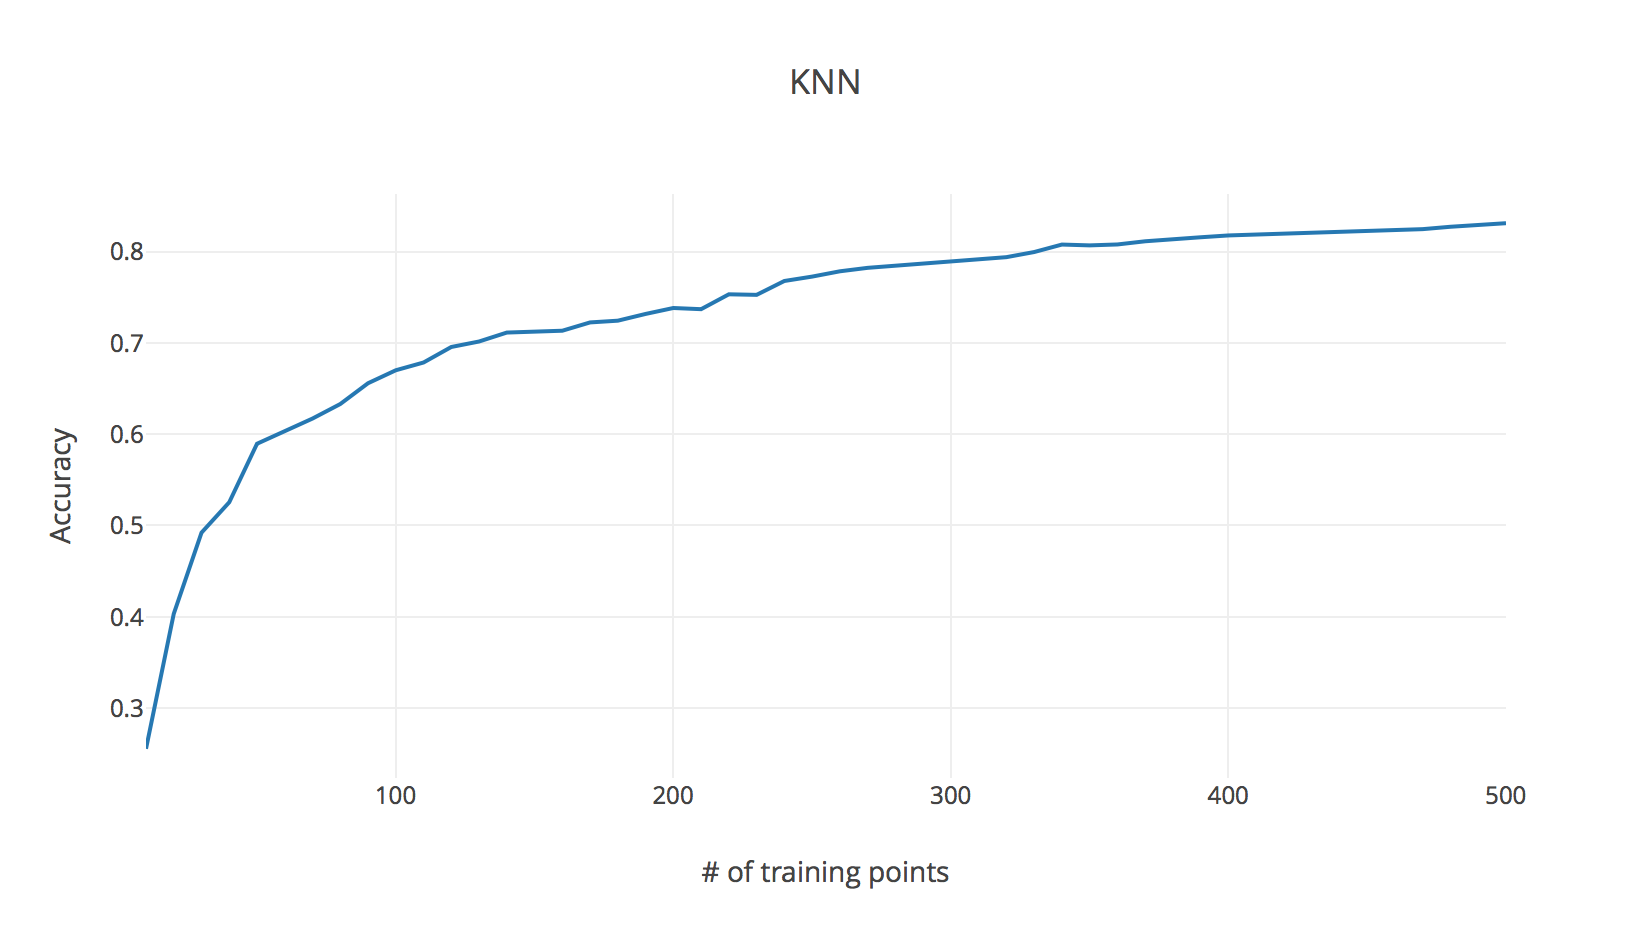
\includegraphics[scale=0.5]{per-limit.png}
  \caption{Accuracy based on the number of training points, I set $k=3$ here.}
\end{figure}

\item \textbf{What is the role of $k$ to accuracy?}

Generally, I had two observations (Figure 2 and 3). First, the parity of $k$ is very important. That is, for odd values of $k$, the accuracy is generally higher than the even values. This makes sense since we use median in case of a tie, which is not a very wise thing to do. Second, small values of $k$ seem to work better.

\begin{figure}[h!]
  \centering
  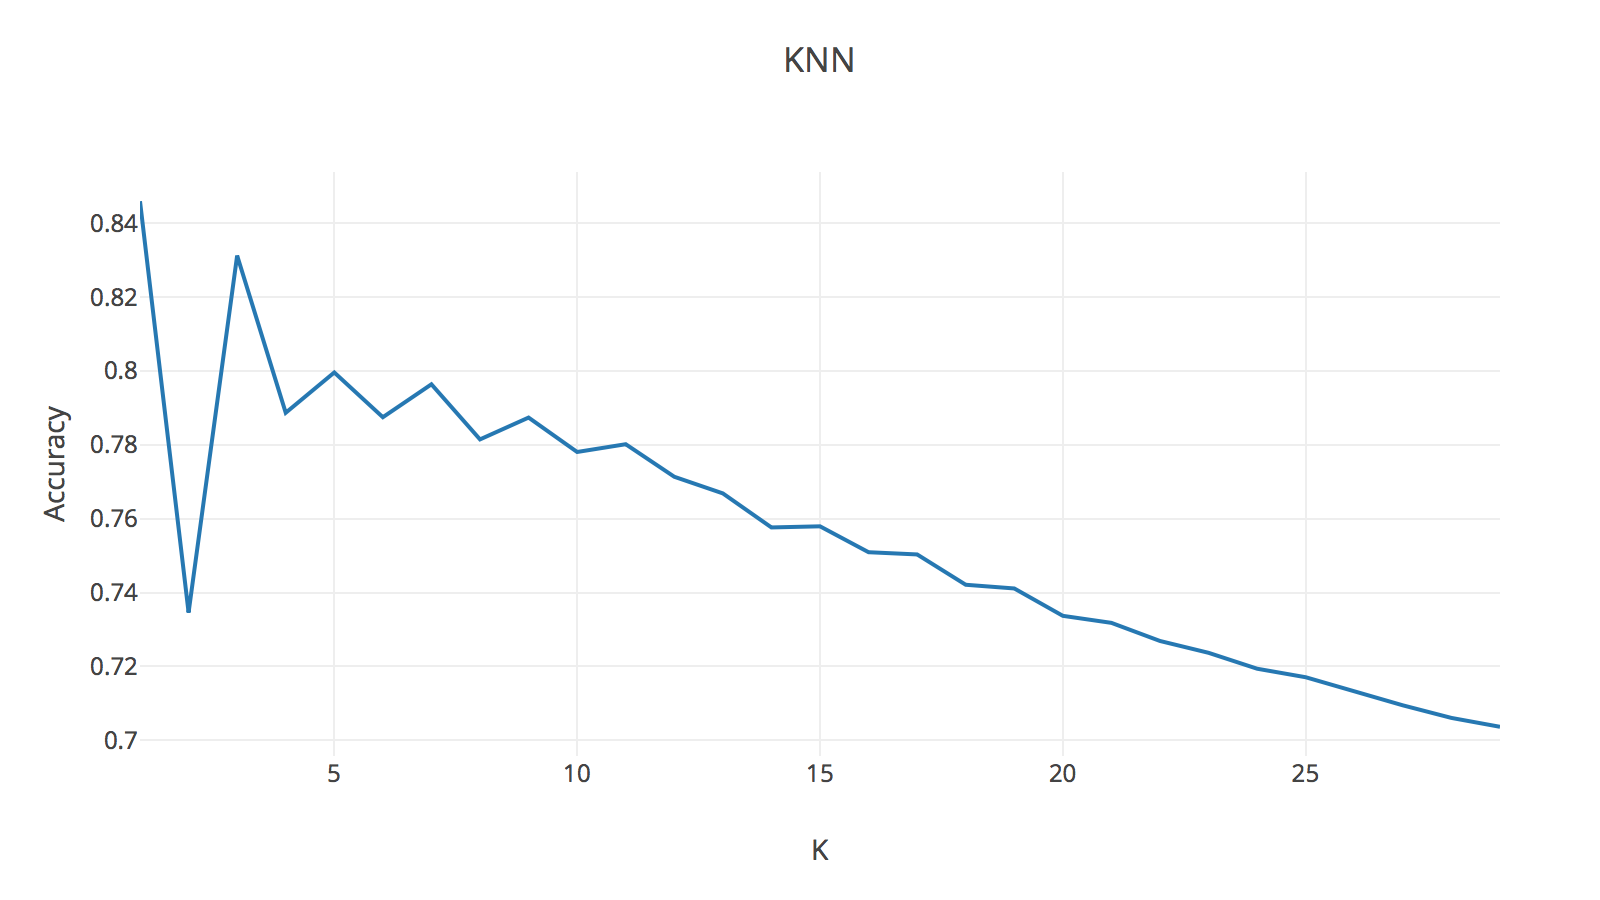
\includegraphics[scale=0.5]{per-k.png}
  \caption{The importance of the parity of $k$ in accuracy is clearly illustrated in the plot. The number of data points here is 500.}
\end{figure}

\begin{figure}[h!]
  \centering
  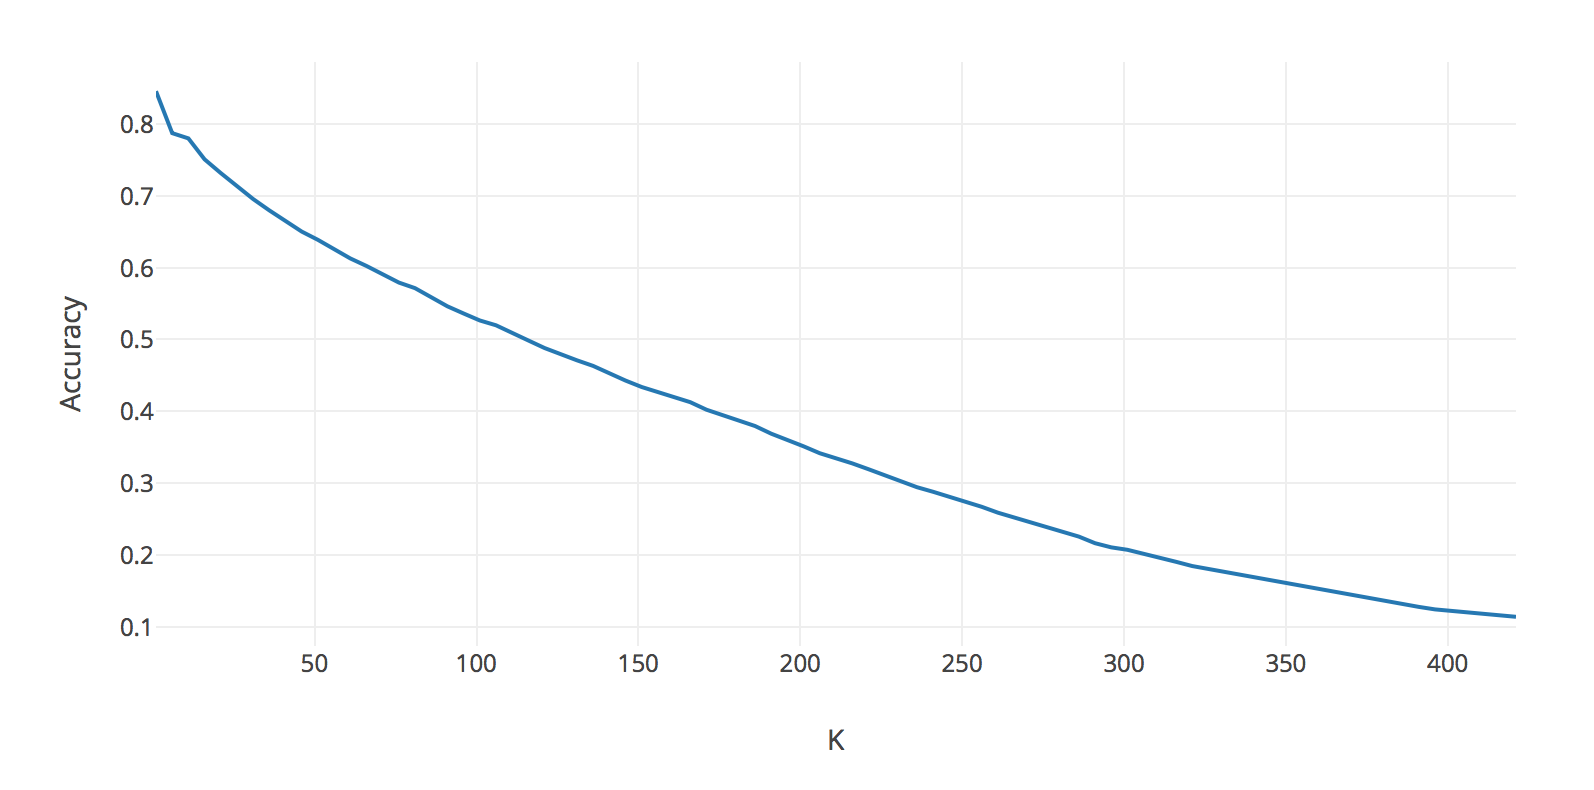
\includegraphics[scale=0.5]{per-k-large.png}
  \caption{The same figure as Figure 2, which also includes larger values of $k$ up to 450. Roughly speaking, the higher $k$ is, the lower is the accuracy. The number of data points here is 500.}
\end{figure}

\item \textbf{What numbers get confused with each other most easily?}

The heat-map in Figure 4 visualizes the confusion matrix. For clarity, I just removed the main diagonal of the matrix. Our classifier is most confused with number 4 and guesses it to be 9. It also quite often guesses 7, 5, and 2 to be 9, 3 and 1 respectively. I also find it interesting that the reverse is not necessarily true, e.g., it doesn't guess 9 to be 4 that much.

\begin{figure}[h!]
  \centering
  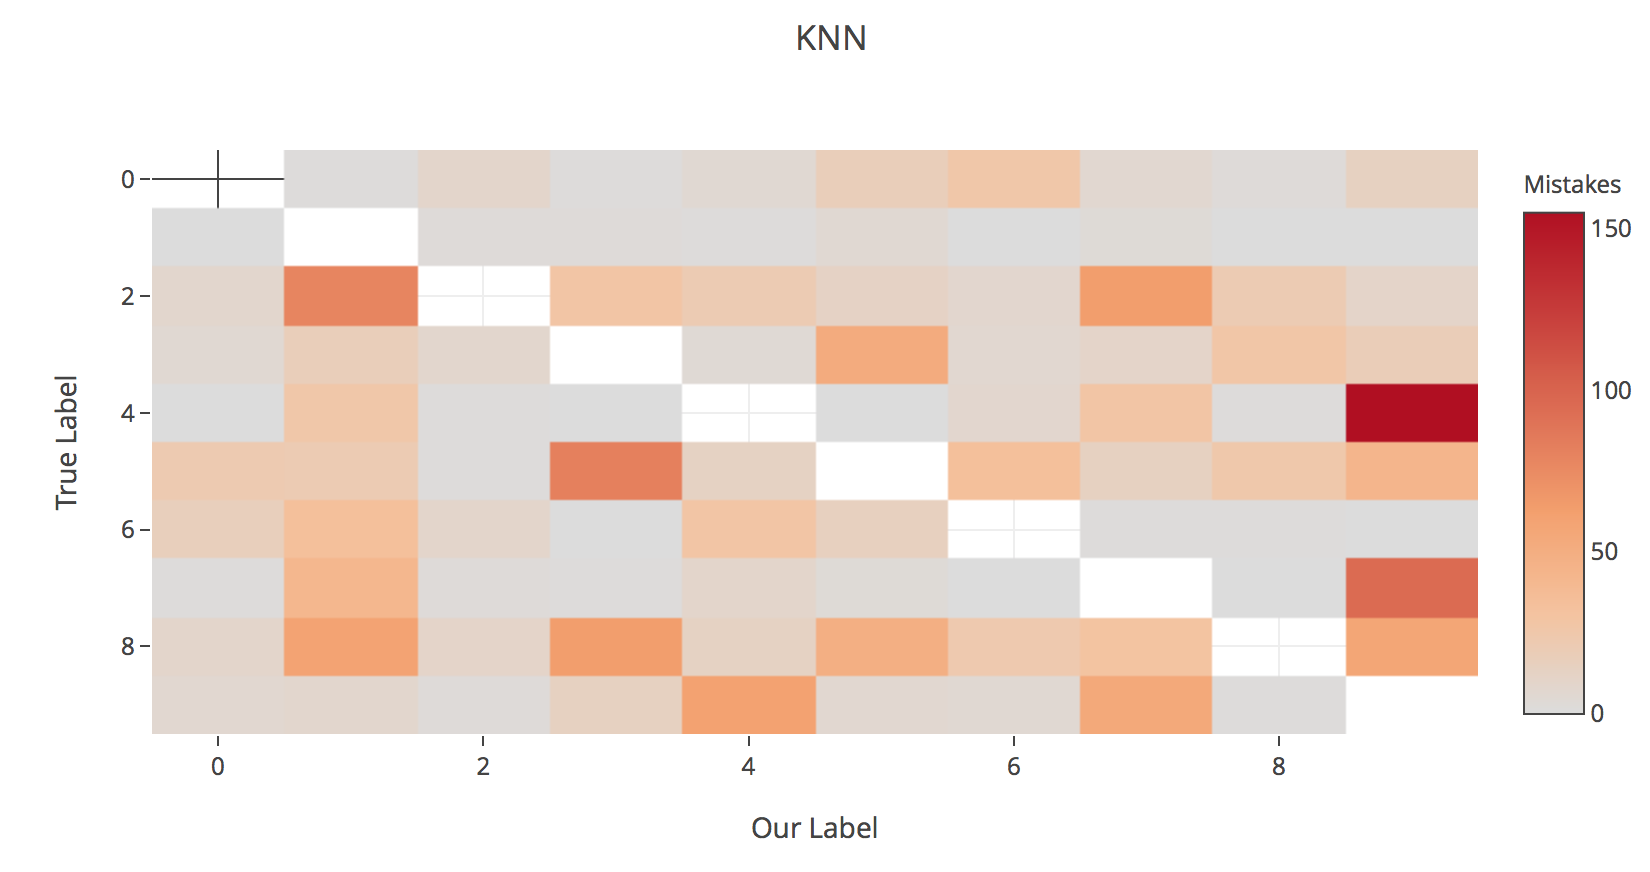
\includegraphics[scale=0.6]{confusion.png}
  \caption{The confusion matrix visualized in a heat-map. The main diagonal was removed to make comparisons easier. The number of data points here is 500 and $k$ is 3.}
\end{figure}

\end{enumerate}

\end{document}
